\documentclass{IOS-Book-Article}
\usepackage{mathptmx}
\usepackage{graphicx}
\usepackage{booktabs}
\usepackage{amsmath}
% generated by src/emit_macros.py; do not edit by hand
\newcommand{\existQwenBase}{0.924}
\newcommand{\strictQwenBase}{0.175}
\newcommand{\existQwenQuota}{0.867}
\newcommand{\strictQwenQuota}{0.165}
\newcommand{\existQwenTemporal}{0.840}
\newcommand{\strictQwenTemporal}{0.081}
\newcommand{\violQwenTemporal}{20}
\newcommand{\existQwenStakes}{0.886}
\newcommand{\strictQwenStakes}{0.145}
\newcommand{\existQwenCombo}{0.773}
\newcommand{\strictQwenCombo}{0.072}
\newcommand{\violQwenCombo}{22}
\newcommand{\loopQwenTrueStart}{0.099}
\newcommand{\loopQwenTrueFinal}{0.107}
\newcommand{\convQwenTrue}{0}
\newcommand{\loopQwenScrStart}{0.099}
\newcommand{\loopQwenScrFinal}{0.093}
\newcommand{\convQwenScr}{0}
\newcommand{\loopQwenNoneStart}{0.099}
\newcommand{\loopQwenNoneFinal}{0.072}
\newcommand{\convQwenNone}{0}
\newcommand{\orCiteQwenQuota}{0.56}
\newcommand{\ciCiteQwenQuota}{0.41 to 0.75}
\newcommand{\pCiteQwenQuota}{0.0001}
\newcommand{\sigCiteQwenQuota}{*}
\newcommand{\orCiteQwenTemporal}{0.45}
\newcommand{\ciCiteQwenTemporal}{0.27 to 0.74}
\newcommand{\pCiteQwenTemporal}{0.0017}
\newcommand{\sigCiteQwenTemporal}{*}
\newcommand{\orCiteQwenStakes}{0.65}
\newcommand{\ciCiteQwenStakes}{0.44 to 0.95}
\newcommand{\pCiteQwenStakes}{0.0255}
\newcommand{\sigCiteQwenStakes}{*}
\newcommand{\orCiteQwenCombo}{0.30}
\newcommand{\ciCiteQwenCombo}{0.18 to 0.51}
\newcommand{\pCiteQwenCombo}{<0.0001}
\newcommand{\sigCiteQwenCombo}{*}
\newcommand{\orQuoteQwenQuota}{0.88}
\newcommand{\ciQuoteQwenQuota}{0.67 to 1.16}
\newcommand{\pQuoteQwenQuota}{0.3570}
\newcommand{\sigQuoteQwenQuota}{}
\newcommand{\orQuoteQwenTemporal}{0.45}
\newcommand{\ciQuoteQwenTemporal}{0.27 to 0.75}
\newcommand{\pQuoteQwenTemporal}{0.0022}
\newcommand{\sigQuoteQwenTemporal}{*}
\newcommand{\orQuoteQwenStakes}{0.78}
\newcommand{\ciQuoteQwenStakes}{0.49 to 1.24}
\newcommand{\pQuoteQwenStakes}{0.2960}
\newcommand{\sigQuoteQwenStakes}{}
\newcommand{\orQuoteQwenCombo}{0.35}
\newcommand{\ciQuoteQwenCombo}{0.24 to 0.52}
\newcommand{\pQuoteQwenCombo}{<0.0001}
\newcommand{\sigQuoteQwenCombo}{*}
\newcommand{\pinAtQwen}{58}
\newcommand{\pinWrongQwen}{35}
\newcommand{\existMistralBase}{0.901}
\newcommand{\strictMistralBase}{0.207}
\newcommand{\existMistralQuota}{0.929}
\newcommand{\strictMistralQuota}{0.261}
\newcommand{\existMistralTemporal}{0.860}
\newcommand{\strictMistralTemporal}{0.117}
\newcommand{\violMistralTemporal}{35}
\newcommand{\existMistralStakes}{0.919}
\newcommand{\strictMistralStakes}{0.167}
\newcommand{\existMistralCombo}{0.868}
\newcommand{\strictMistralCombo}{0.136}
\newcommand{\violMistralCombo}{37}
\newcommand{\loopMistralTrueStart}{0.208}
\newcommand{\loopMistralTrueFinal}{0.264}
\newcommand{\convMistralTrue}{9}
\newcommand{\loopMistralScrStart}{0.208}
\newcommand{\loopMistralScrFinal}{0.122}
\newcommand{\convMistralScr}{3}
\newcommand{\loopMistralNoneStart}{0.208}
\newcommand{\loopMistralNoneFinal}{0.198}
\newcommand{\convMistralNone}{3}
\newcommand{\orCiteMistralQuota}{1.41}
\newcommand{\ciCiteMistralQuota}{0.96 to 2.08}
\newcommand{\pCiteMistralQuota}{0.0825}
\newcommand{\sigCiteMistralQuota}{}
\newcommand{\orCiteMistralTemporal}{0.68}
\newcommand{\ciCiteMistralTemporal}{0.45 to 1.01}
\newcommand{\pCiteMistralTemporal}{0.0575}
\newcommand{\sigCiteMistralTemporal}{}
\newcommand{\orCiteMistralStakes}{1.27}
\newcommand{\ciCiteMistralStakes}{0.75 to 2.16}
\newcommand{\pCiteMistralStakes}{0.3748}
\newcommand{\sigCiteMistralStakes}{}
\newcommand{\orCiteMistralCombo}{0.75}
\newcommand{\ciCiteMistralCombo}{0.49 to 1.13}
\newcommand{\pCiteMistralCombo}{0.1649}
\newcommand{\sigCiteMistralCombo}{}
\newcommand{\orQuoteMistralQuota}{1.42}
\newcommand{\ciQuoteMistralQuota}{0.92 to 2.19}
\newcommand{\pQuoteMistralQuota}{0.1128}
\newcommand{\sigQuoteMistralQuota}{}
\newcommand{\orQuoteMistralTemporal}{0.50}
\newcommand{\ciQuoteMistralTemporal}{0.30 to 0.83}
\newcommand{\pQuoteMistralTemporal}{0.0075}
\newcommand{\sigQuoteMistralTemporal}{*}
\newcommand{\orQuoteMistralStakes}{0.83}
\newcommand{\ciQuoteMistralStakes}{0.52 to 1.32}
\newcommand{\pQuoteMistralStakes}{0.4277}
\newcommand{\sigQuoteMistralStakes}{}
\newcommand{\orQuoteMistralCombo}{0.67}
\newcommand{\ciQuoteMistralCombo}{0.40 to 1.12}
\newcommand{\pQuoteMistralCombo}{0.1254}
\newcommand{\sigQuoteMistralCombo}{}
\newcommand{\pinAtMistral}{42}
\newcommand{\pinWrongMistral}{45}
\newcommand{\existLlamaBase}{0.958}
\newcommand{\strictLlamaBase}{0.402}
\newcommand{\existLlamaQuota}{0.975}
\newcommand{\strictLlamaQuota}{0.327}
\newcommand{\existLlamaTemporal}{0.944}
\newcommand{\strictLlamaTemporal}{0.139}
\newcommand{\violLlamaTemporal}{10}
\newcommand{\existLlamaStakes}{0.956}
\newcommand{\strictLlamaStakes}{0.380}
\newcommand{\existLlamaCombo}{0.939}
\newcommand{\strictLlamaCombo}{0.179}
\newcommand{\violLlamaCombo}{9}
\newcommand{\loopLlamaTrueStart}{0.176}
\newcommand{\loopLlamaTrueFinal}{0.349}
\newcommand{\convLlamaTrue}{21}
\newcommand{\loopLlamaScrStart}{0.176}
\newcommand{\loopLlamaScrFinal}{0.188}
\newcommand{\convLlamaScr}{6}
\newcommand{\loopLlamaNoneStart}{0.176}
\newcommand{\loopLlamaNoneFinal}{0.109}
\newcommand{\convLlamaNone}{7}
\newcommand{\orCiteLlamaQuota}{1.54}
\newcommand{\ciCiteLlamaQuota}{0.79 to 3.00}
\newcommand{\pCiteLlamaQuota}{0.2071}
\newcommand{\sigCiteLlamaQuota}{}
\newcommand{\orCiteLlamaTemporal}{0.73}
\newcommand{\ciCiteLlamaTemporal}{0.29 to 1.82}
\newcommand{\pCiteLlamaTemporal}{0.4954}
\newcommand{\sigCiteLlamaTemporal}{}
\newcommand{\orCiteLlamaStakes}{0.90}
\newcommand{\ciCiteLlamaStakes}{0.34 to 2.35}
\newcommand{\pCiteLlamaStakes}{0.8262}
\newcommand{\sigCiteLlamaStakes}{}
\newcommand{\orCiteLlamaCombo}{0.70}
\newcommand{\ciCiteLlamaCombo}{0.34 to 1.45}
\newcommand{\pCiteLlamaCombo}{0.3313}
\newcommand{\sigCiteLlamaCombo}{}
\newcommand{\orQuoteLlamaQuota}{0.69}
\newcommand{\ciQuoteLlamaQuota}{0.45 to 1.06}
\newcommand{\pQuoteLlamaQuota}{0.0914}
\newcommand{\sigQuoteLlamaQuota}{}
\newcommand{\orQuoteLlamaTemporal}{0.20}
\newcommand{\ciQuoteLlamaTemporal}{0.10 to 0.40}
\newcommand{\pQuoteLlamaTemporal}{<0.0001}
\newcommand{\sigQuoteLlamaTemporal}{*}
\newcommand{\orQuoteLlamaStakes}{0.87}
\newcommand{\ciQuoteLlamaStakes}{0.52 to 1.46}
\newcommand{\pQuoteLlamaStakes}{0.6052}
\newcommand{\sigQuoteLlamaStakes}{}
\newcommand{\orQuoteLlamaCombo}{0.26}
\newcommand{\ciQuoteLlamaCombo}{0.14 to 0.50}
\newcommand{\pQuoteLlamaCombo}{<0.0001}
\newcommand{\sigQuoteLlamaCombo}{*}
\newcommand{\pinAtLlama}{64}
\newcommand{\pinWrongLlama}{27}
\newcommand{\existDeepseekBase}{0.972}
\newcommand{\strictDeepseekBase}{0.281}
\newcommand{\existDeepseekQuota}{0.950}
\newcommand{\strictDeepseekQuota}{0.266}
\newcommand{\existDeepseekTemporal}{0.952}
\newcommand{\strictDeepseekTemporal}{0.187}
\newcommand{\violDeepseekTemporal}{11}
\newcommand{\existDeepseekStakes}{0.967}
\newcommand{\strictDeepseekStakes}{0.270}
\newcommand{\existDeepseekCombo}{0.959}
\newcommand{\strictDeepseekCombo}{0.120}
\newcommand{\violDeepseekCombo}{7}
\newcommand{\loopDeepseekTrueStart}{0.181}
\newcommand{\loopDeepseekTrueFinal}{0.645}
\newcommand{\convDeepseekTrue}{21}
\newcommand{\loopDeepseekScrStart}{0.181}
\newcommand{\loopDeepseekScrFinal}{0.153}
\newcommand{\convDeepseekScr}{4}
\newcommand{\loopDeepseekNoneStart}{0.181}
\newcommand{\loopDeepseekNoneFinal}{0.152}
\newcommand{\convDeepseekNone}{0}
\newcommand{\orCiteDeepseekQuota}{0.64}
\newcommand{\ciCiteDeepseekQuota}{0.35 to 1.15}
\newcommand{\pCiteDeepseekQuota}{0.1359}
\newcommand{\sigCiteDeepseekQuota}{}
\newcommand{\orCiteDeepseekTemporal}{0.62}
\newcommand{\ciCiteDeepseekTemporal}{0.27 to 1.45}
\newcommand{\pCiteDeepseekTemporal}{0.2685}
\newcommand{\sigCiteDeepseekTemporal}{}
\newcommand{\orCiteDeepseekStakes}{0.91}
\newcommand{\ciCiteDeepseekStakes}{0.38 to 2.17}
\newcommand{\pCiteDeepseekStakes}{0.8308}
\newcommand{\sigCiteDeepseekStakes}{}
\newcommand{\orCiteDeepseekCombo}{0.79}
\newcommand{\ciCiteDeepseekCombo}{0.34 to 1.82}
\newcommand{\pCiteDeepseekCombo}{0.5760}
\newcommand{\sigCiteDeepseekCombo}{}
\newcommand{\orQuoteDeepseekQuota}{0.96}
\newcommand{\ciQuoteDeepseekQuota}{0.68 to 1.35}
\newcommand{\pQuoteDeepseekQuota}{0.8175}
\newcommand{\sigQuoteDeepseekQuota}{}
\newcommand{\orQuoteDeepseekTemporal}{0.61}
\newcommand{\ciQuoteDeepseekTemporal}{0.40 to 0.94}
\newcommand{\pQuoteDeepseekTemporal}{0.0251}
\newcommand{\sigQuoteDeepseekTemporal}{*}
\newcommand{\orQuoteDeepseekStakes}{0.96}
\newcommand{\ciQuoteDeepseekStakes}{0.65 to 1.43}
\newcommand{\pQuoteDeepseekStakes}{0.8463}
\newcommand{\sigQuoteDeepseekStakes}{}
\newcommand{\orQuoteDeepseekCombo}{0.39}
\newcommand{\ciQuoteDeepseekCombo}{0.27 to 0.56}
\newcommand{\pQuoteDeepseekCombo}{<0.0001}
\newcommand{\sigQuoteDeepseekCombo}{*}
\newcommand{\pinAtDeepseek}{58}
\newcommand{\pinWrongDeepseek}{25}
\newcommand{\existGptBase}{0.981}
\newcommand{\strictGptBase}{0.460}
\newcommand{\existGptQuota}{0.981}
\newcommand{\strictGptQuota}{0.454}
\newcommand{\existGptTemporal}{0.958}
\newcommand{\strictGptTemporal}{0.323}
\newcommand{\violGptTemporal}{13}
\newcommand{\existGptStakes}{0.979}
\newcommand{\strictGptStakes}{0.422}
\newcommand{\existGptCombo}{0.962}
\newcommand{\strictGptCombo}{0.294}
\newcommand{\violGptCombo}{14}
\newcommand{\loopGptTrueStart}{0.360}
\newcommand{\loopGptTrueFinal}{0.719}
\newcommand{\convGptTrue}{22}
\newcommand{\loopGptScrStart}{0.360}
\newcommand{\loopGptScrFinal}{0.241}
\newcommand{\convGptScr}{6}
\newcommand{\loopGptNoneStart}{0.360}
\newcommand{\loopGptNoneFinal}{0.543}
\newcommand{\convGptNone}{13}
\newcommand{\orCiteGptQuota}{1.07}
\newcommand{\ciCiteGptQuota}{0.47 to 2.45}
\newcommand{\pCiteGptQuota}{0.8781}
\newcommand{\sigCiteGptQuota}{}
\newcommand{\orCiteGptTemporal}{0.49}
\newcommand{\ciCiteGptTemporal}{0.20 to 1.18}
\newcommand{\pCiteGptTemporal}{0.1133}
\newcommand{\sigCiteGptTemporal}{}
\newcommand{\orCiteGptStakes}{0.97}
\newcommand{\ciCiteGptStakes}{0.48 to 1.98}
\newcommand{\pCiteGptStakes}{0.9414}
\newcommand{\sigCiteGptStakes}{}
\newcommand{\orCiteGptCombo}{0.55}
\newcommand{\ciCiteGptCombo}{0.28 to 1.08}
\newcommand{\pCiteGptCombo}{0.0835}
\newcommand{\sigCiteGptCombo}{}
\newcommand{\orQuoteGptQuota}{0.96}
\newcommand{\ciQuoteGptQuota}{0.60 to 1.54}
\newcommand{\pQuoteGptQuota}{0.8564}
\newcommand{\sigQuoteGptQuota}{}
\newcommand{\orQuoteGptTemporal}{0.55}
\newcommand{\ciQuoteGptTemporal}{0.30 to 1.00}
\newcommand{\pQuoteGptTemporal}{0.0488}
\newcommand{\sigQuoteGptTemporal}{*}
\newcommand{\orQuoteGptStakes}{0.84}
\newcommand{\ciQuoteGptStakes}{0.55 to 1.29}
\newcommand{\pQuoteGptStakes}{0.4374}
\newcommand{\sigQuoteGptStakes}{}
\newcommand{\orQuoteGptCombo}{0.46}
\newcommand{\ciQuoteGptCombo}{0.23 to 0.90}
\newcommand{\pQuoteGptCombo}{0.0233}
\newcommand{\sigQuoteGptCombo}{*}
\newcommand{\pinAtGpt}{51}
\newcommand{\pinWrongGpt}{31}
\newcommand{\existSonnetBase}{0.991}
\newcommand{\strictSonnetBase}{0.333}
\newcommand{\existSonnetQuota}{0.985}
\newcommand{\strictSonnetQuota}{0.333}
\newcommand{\existSonnetTemporal}{0.994}
\newcommand{\strictSonnetTemporal}{0.374}
\newcommand{\violSonnetTemporal}{0}
\newcommand{\existSonnetStakes}{0.991}
\newcommand{\strictSonnetStakes}{0.390}
\newcommand{\existSonnetCombo}{0.998}
\newcommand{\strictSonnetCombo}{0.427}
\newcommand{\violSonnetCombo}{0}
\newcommand{\loopSonnetTrueStart}{0.471}
\newcommand{\loopSonnetTrueFinal}{0.974}
\newcommand{\convSonnetTrue}{23}
\newcommand{\loopSonnetScrStart}{0.471}
\newcommand{\loopSonnetScrFinal}{0.266}
\newcommand{\convSonnetScr}{4}
\newcommand{\loopSonnetNoneStart}{0.471}
\newcommand{\loopSonnetNoneFinal}{0.595}
\newcommand{\convSonnetNone}{6}
\newcommand{\orCiteSonnetQuota}{0.64}
\newcommand{\ciCiteSonnetQuota}{0.26 to 1.59}
\newcommand{\pCiteSonnetQuota}{0.3345}
\newcommand{\sigCiteSonnetQuota}{}
\newcommand{\orCiteSonnetTemporal}{1.92}
\newcommand{\ciCiteSonnetTemporal}{0.89 to 4.13}
\newcommand{\pCiteSonnetTemporal}{0.0942}
\newcommand{\sigCiteSonnetTemporal}{}
\newcommand{\orCiteSonnetStakes}{1.20}
\newcommand{\ciCiteSonnetStakes}{0.52 to 2.79}
\newcommand{\pCiteSonnetStakes}{0.6722}
\newcommand{\sigCiteSonnetStakes}{}
\newcommand{\orCiteSonnetCombo}{4.56}
\newcommand{\ciCiteSonnetCombo}{1.12 to 18.45}
\newcommand{\pCiteSonnetCombo}{0.0336}
\newcommand{\sigCiteSonnetCombo}{*}
\newcommand{\orQuoteSonnetQuota}{0.99}
\newcommand{\ciQuoteSonnetQuota}{0.76 to 1.30}
\newcommand{\pQuoteSonnetQuota}{0.9589}
\newcommand{\sigQuoteSonnetQuota}{}
\newcommand{\orQuoteSonnetTemporal}{1.16}
\newcommand{\ciQuoteSonnetTemporal}{0.84 to 1.60}
\newcommand{\pQuoteSonnetTemporal}{0.3801}
\newcommand{\sigQuoteSonnetTemporal}{}
\newcommand{\orQuoteSonnetStakes}{1.28}
\newcommand{\ciQuoteSonnetStakes}{0.90 to 1.81}
\newcommand{\pQuoteSonnetStakes}{0.1648}
\newcommand{\sigQuoteSonnetStakes}{}
\newcommand{\orQuoteSonnetCombo}{1.48}
\newcommand{\ciQuoteSonnetCombo}{1.04 to 2.09}
\newcommand{\pQuoteSonnetCombo}{0.0292}
\newcommand{\sigQuoteSonnetCombo}{*}
\newcommand{\pinAtSonnet}{77}
\newcommand{\pinWrongSonnet}{16}
\newcommand{\humanStrict}{0.407}
\newcommand{\humanScored}{578}
\newcommand{\humanExist}{0.931}
\newcommand{\humanExcerpts}{482}
\newcommand{\nModels}{6}
\newcommand{\nDrafts}{1,440}
\newcommand{\nEpisodes}{288}
\newcommand{\sonnetParaphrase}{413}
\newcommand{\sonnetFabricated}{202}
\newcommand{\sonnetOutOfScope}{131}
\newcommand{\sonnetParaphrasePct}{55}
\newcommand{\nPressured}{1,152}
\newcommand{\nHolmTests}{8}
\newcommand{\humanLenient}{0.680}
\newcommand{\humanNearMissShare}{27}
\newcommand{\holmQuoteDeepseekCombo}{<0.001}
\newcommand{\holmQuoteDeepseekTemporal}{0.176}
\newcommand{\holmCiteDeepseekQuota}{0.815}
\newcommand{\holmCiteDeepseekTemporal}{1.000}
\newcommand{\holmCiteDeepseekCombo}{1.000}
\newcommand{\holmQuoteDeepseekQuota}{1.000}
\newcommand{\holmCiteDeepseekStakes}{1.000}
\newcommand{\holmQuoteDeepseekStakes}{0.846}
\newcommand{\holmQuoteGptCombo}{0.187}
\newcommand{\holmQuoteGptTemporal}{0.341}
\newcommand{\holmCiteGptCombo}{0.501}
\newcommand{\holmCiteGptTemporal}{0.566}
\newcommand{\holmQuoteGptStakes}{1.000}
\newcommand{\holmQuoteGptQuota}{1.000}
\newcommand{\holmCiteGptQuota}{1.000}
\newcommand{\holmCiteGptStakes}{0.941}
\newcommand{\holmQuoteLlamaTemporal}{<0.001}
\newcommand{\holmQuoteLlamaCombo}{<0.001}
\newcommand{\holmQuoteLlamaQuota}{0.549}
\newcommand{\holmCiteLlamaQuota}{1.000}
\newcommand{\holmCiteLlamaCombo}{1.000}
\newcommand{\holmCiteLlamaTemporal}{1.000}
\newcommand{\holmQuoteLlamaStakes}{1.000}
\newcommand{\holmCiteLlamaStakes}{0.826}
\newcommand{\holmQuoteMistralTemporal}{0.060}
\newcommand{\holmCiteMistralTemporal}{0.403}
\newcommand{\holmCiteMistralQuota}{0.495}
\newcommand{\holmQuoteMistralQuota}{0.564}
\newcommand{\holmQuoteMistralCombo}{0.502}
\newcommand{\holmCiteMistralCombo}{0.495}
\newcommand{\holmCiteMistralStakes}{0.750}
\newcommand{\holmQuoteMistralStakes}{0.428}
\newcommand{\holmQuoteQwenCombo}{<0.001}
\newcommand{\holmCiteQwenCombo}{<0.001}
\newcommand{\holmCiteQwenQuota}{<0.001}
\newcommand{\holmCiteQwenTemporal}{0.008}
\newcommand{\holmQuoteQwenTemporal}{0.009}
\newcommand{\holmCiteQwenStakes}{0.076}
\newcommand{\holmQuoteQwenStakes}{0.592}
\newcommand{\holmQuoteQwenQuota}{0.357}
\newcommand{\holmQuoteSonnetCombo}{0.233}
\newcommand{\holmCiteSonnetCombo}{0.235}
\newcommand{\holmCiteSonnetTemporal}{0.565}
\newcommand{\holmQuoteSonnetStakes}{0.824}
\newcommand{\holmCiteSonnetQuota}{1.000}
\newcommand{\holmQuoteSonnetTemporal}{1.000}
\newcommand{\holmCiteSonnetStakes}{1.000}
\newcommand{\holmQuoteSonnetQuota}{0.959}
\newcommand{\lenientDeepseekBase}{0.631}
\newcommand{\lenientDeepseekCombo}{0.436}
\newcommand{\lenientDeepseekQuota}{0.605}
\newcommand{\lenientDeepseekStakes}{0.602}
\newcommand{\lenientDeepseekTemporal}{0.483}
\newcommand{\lenientGptBase}{0.722}
\newcommand{\lenientGptCombo}{0.571}
\newcommand{\lenientGptQuota}{0.747}
\newcommand{\lenientGptStakes}{0.690}
\newcommand{\lenientGptTemporal}{0.573}
\newcommand{\lenientLlamaBase}{0.618}
\newcommand{\lenientLlamaCombo}{0.453}
\newcommand{\lenientLlamaQuota}{0.667}
\newcommand{\lenientLlamaStakes}{0.685}
\newcommand{\lenientLlamaTemporal}{0.430}
\newcommand{\lenientMistralBase}{0.608}
\newcommand{\lenientMistralCombo}{0.383}
\newcommand{\lenientMistralQuota}{0.581}
\newcommand{\lenientMistralStakes}{0.567}
\newcommand{\lenientMistralTemporal}{0.438}
\newcommand{\lenientQwenBase}{0.564}
\newcommand{\lenientQwenCombo}{0.320}
\newcommand{\lenientQwenQuota}{0.578}
\newcommand{\lenientQwenStakes}{0.592}
\newcommand{\lenientQwenTemporal}{0.315}
\newcommand{\lenientSonnetBase}{0.622}
\newcommand{\lenientSonnetCombo}{0.642}
\newcommand{\lenientSonnetQuota}{0.612}
\newcommand{\lenientSonnetStakes}{0.586}
\newcommand{\lenientSonnetTemporal}{0.608}
\newcommand{\lqScoredDeepseekTrueStart}{211}
\newcommand{\lqScoredDeepseekTrueFinal}{47}
\newcommand{\lqAccDeepseekTrueStart}{28}
\newcommand{\lqAccDeepseekTrueFinal}{19}
\newcommand{\lCitesDeepseekTrueStart}{248}
\newcommand{\lCitesDeepseekTrueFinal}{236}
\newcommand{\lExistDeepseekTrueStart}{0.971}
\newcommand{\lExistDeepseekTrueFinal}{1.000}
\newcommand{\lqScoredDeepseekScrStart}{211}
\newcommand{\lqScoredDeepseekScrFinal}{105}
\newcommand{\lqAccDeepseekScrStart}{28}
\newcommand{\lqAccDeepseekScrFinal}{7}
\newcommand{\lCitesDeepseekScrStart}{248}
\newcommand{\lCitesDeepseekScrFinal}{191}
\newcommand{\lExistDeepseekScrStart}{0.971}
\newcommand{\lExistDeepseekScrFinal}{0.960}
\newcommand{\lqScoredDeepseekNoneStart}{211}
\newcommand{\lqScoredDeepseekNoneFinal}{185}
\newcommand{\lqAccDeepseekNoneStart}{28}
\newcommand{\lqAccDeepseekNoneFinal}{26}
\newcommand{\lCitesDeepseekNoneStart}{248}
\newcommand{\lCitesDeepseekNoneFinal}{248}
\newcommand{\lExistDeepseekNoneStart}{0.971}
\newcommand{\lExistDeepseekNoneFinal}{0.969}
\newcommand{\lqScoredGptTrueStart}{65}
\newcommand{\lqScoredGptTrueFinal}{39}
\newcommand{\lqAccGptTrueStart}{28}
\newcommand{\lqAccGptTrueFinal}{29}
\newcommand{\lCitesGptTrueStart}{366}
\newcommand{\lCitesGptTrueFinal}{354}
\newcommand{\lExistGptTrueStart}{0.959}
\newcommand{\lExistGptTrueFinal}{0.996}
\newcommand{\lqScoredGptScrStart}{65}
\newcommand{\lqScoredGptScrFinal}{41}
\newcommand{\lqAccGptScrStart}{28}
\newcommand{\lqAccGptScrFinal}{15}
\newcommand{\lCitesGptScrStart}{366}
\newcommand{\lCitesGptScrFinal}{331}
\newcommand{\lExistGptScrStart}{0.959}
\newcommand{\lExistGptScrFinal}{0.937}
\newcommand{\lqScoredGptNoneStart}{65}
\newcommand{\lqScoredGptNoneFinal}{38}
\newcommand{\lqAccGptNoneStart}{28}
\newcommand{\lqAccGptNoneFinal}{21}
\newcommand{\lCitesGptNoneStart}{366}
\newcommand{\lCitesGptNoneFinal}{306}
\newcommand{\lExistGptNoneStart}{0.959}
\newcommand{\lExistGptNoneFinal}{0.975}
\newcommand{\lqScoredLlamaTrueStart}{64}
\newcommand{\lqScoredLlamaTrueFinal}{29}
\newcommand{\lqAccLlamaTrueStart}{11}
\newcommand{\lqAccLlamaTrueFinal}{8}
\newcommand{\lCitesLlamaTrueStart}{270}
\newcommand{\lCitesLlamaTrueFinal}{244}
\newcommand{\lExistLlamaTrueStart}{0.930}
\newcommand{\lExistLlamaTrueFinal}{1.000}
\newcommand{\lqScoredLlamaScrStart}{64}
\newcommand{\lqScoredLlamaScrFinal}{35}
\newcommand{\lqAccLlamaScrStart}{11}
\newcommand{\lqAccLlamaScrFinal}{6}
\newcommand{\lCitesLlamaScrStart}{270}
\newcommand{\lCitesLlamaScrFinal}{221}
\newcommand{\lExistLlamaScrStart}{0.930}
\newcommand{\lExistLlamaScrFinal}{0.849}
\newcommand{\lqScoredLlamaNoneStart}{64}
\newcommand{\lqScoredLlamaNoneFinal}{32}
\newcommand{\lqAccLlamaNoneStart}{11}
\newcommand{\lqAccLlamaNoneFinal}{3}
\newcommand{\lCitesLlamaNoneStart}{270}
\newcommand{\lCitesLlamaNoneFinal}{235}
\newcommand{\lExistLlamaNoneStart}{0.930}
\newcommand{\lExistLlamaNoneFinal}{0.943}
\newcommand{\lqScoredMistralTrueStart}{145}
\newcommand{\lqScoredMistralTrueFinal}{133}
\newcommand{\lqAccMistralTrueStart}{15}
\newcommand{\lqAccMistralTrueFinal}{17}
\newcommand{\lCitesMistralTrueStart}{267}
\newcommand{\lCitesMistralTrueFinal}{261}
\newcommand{\lExistMistralTrueStart}{0.877}
\newcommand{\lExistMistralTrueFinal}{0.961}
\newcommand{\lqScoredMistralScrStart}{145}
\newcommand{\lqScoredMistralScrFinal}{136}
\newcommand{\lqAccMistralScrStart}{15}
\newcommand{\lqAccMistralScrFinal}{12}
\newcommand{\lCitesMistralScrStart}{267}
\newcommand{\lCitesMistralScrFinal}{268}
\newcommand{\lExistMistralScrStart}{0.877}
\newcommand{\lExistMistralScrFinal}{0.834}
\newcommand{\lqScoredMistralNoneStart}{145}
\newcommand{\lqScoredMistralNoneFinal}{144}
\newcommand{\lqAccMistralNoneStart}{15}
\newcommand{\lqAccMistralNoneFinal}{19}
\newcommand{\lCitesMistralNoneStart}{267}
\newcommand{\lCitesMistralNoneFinal}{261}
\newcommand{\lExistMistralNoneStart}{0.877}
\newcommand{\lExistMistralNoneFinal}{0.883}
\newcommand{\lqScoredQwenTrueStart}{186}
\newcommand{\lqScoredQwenTrueFinal}{188}
\newcommand{\lqAccQwenTrueStart}{16}
\newcommand{\lqAccQwenTrueFinal}{16}
\newcommand{\lCitesQwenTrueStart}{198}
\newcommand{\lCitesQwenTrueFinal}{197}
\newcommand{\lExistQwenTrueStart}{0.739}
\newcommand{\lExistQwenTrueFinal}{0.822}
\newcommand{\lqScoredQwenScrStart}{186}
\newcommand{\lqScoredQwenScrFinal}{166}
\newcommand{\lqAccQwenScrStart}{16}
\newcommand{\lqAccQwenScrFinal}{12}
\newcommand{\lCitesQwenScrStart}{198}
\newcommand{\lCitesQwenScrFinal}{206}
\newcommand{\lExistQwenScrStart}{0.739}
\newcommand{\lExistQwenScrFinal}{0.685}
\newcommand{\lqScoredQwenNoneStart}{186}
\newcommand{\lqScoredQwenNoneFinal}{185}
\newcommand{\lqAccQwenNoneStart}{16}
\newcommand{\lqAccQwenNoneFinal}{14}
\newcommand{\lCitesQwenNoneStart}{198}
\newcommand{\lCitesQwenNoneFinal}{195}
\newcommand{\lExistQwenNoneStart}{0.739}
\newcommand{\lExistQwenNoneFinal}{0.751}
\newcommand{\lqScoredSonnetTrueStart}{157}
\newcommand{\lqScoredSonnetTrueFinal}{73}
\newcommand{\lqAccSonnetTrueStart}{68}
\newcommand{\lqAccSonnetTrueFinal}{70}
\newcommand{\lCitesSonnetTrueStart}{220}
\newcommand{\lCitesSonnetTrueFinal}{220}
\newcommand{\lExistSonnetTrueStart}{1.000}
\newcommand{\lExistSonnetTrueFinal}{1.000}
\newcommand{\lqScoredSonnetScrStart}{157}
\newcommand{\lqScoredSonnetScrFinal}{69}
\newcommand{\lqAccSonnetScrStart}{68}
\newcommand{\lqAccSonnetScrFinal}{26}
\newcommand{\lCitesSonnetScrStart}{220}
\newcommand{\lCitesSonnetScrFinal}{203}
\newcommand{\lExistSonnetScrStart}{1.000}
\newcommand{\lExistSonnetScrFinal}{1.000}
\newcommand{\lqScoredSonnetNoneStart}{157}
\newcommand{\lqScoredSonnetNoneFinal}{138}
\newcommand{\lqAccSonnetNoneStart}{68}
\newcommand{\lqAccSonnetNoneFinal}{74}
\newcommand{\lCitesSonnetNoneStart}{220}
\newcommand{\lCitesSonnetNoneFinal}{230}
\newcommand{\lExistSonnetNoneStart}{1.000}
\newcommand{\lExistSonnetNoneFinal}{1.000}
\newcommand{\ldiffDeepseekScr}{0.39}
\newcommand{\lciDeepseekScr}{0.16 to 0.62}
\newcommand{\lpDeepseekScr}{0.016}
\newcommand{\lnDeepseekScr}{14}
\newcommand{\ldiffDeepseekNone}{0.49}
\newcommand{\lciDeepseekNone}{0.27 to 0.70}
\newcommand{\lpDeepseekNone}{0.005}
\newcommand{\lnDeepseekNone}{15}
\newcommand{\ldiffGptScr}{0.44}
\newcommand{\lciGptScr}{0.23 to 0.66}
\newcommand{\lpGptScr}{0.004}
\newcommand{\lnGptScr}{17}
\newcommand{\ldiffGptNone}{0.12}
\newcommand{\lciGptNone}{-0.06 to 0.32}
\newcommand{\lpGptNone}{0.293}
\newcommand{\lnGptNone}{13}
\newcommand{\ldiffLlamaScr}{0.03}
\newcommand{\lciLlamaScr}{-0.14 to 0.17}
\newcommand{\lpLlamaScr}{0.713}
\newcommand{\lnLlamaScr}{13}
\newcommand{\ldiffLlamaNone}{0.29}
\newcommand{\lciLlamaNone}{0.08 to 0.53}
\newcommand{\lpLlamaNone}{0.039}
\newcommand{\lnLlamaNone}{13}
\newcommand{\ldiffMistralScr}{0.12}
\newcommand{\lciMistralScr}{0.05 to 0.21}
\newcommand{\lpMistralScr}{0.012}
\newcommand{\lnMistralScr}{18}
\newcommand{\ldiffMistralNone}{0.03}
\newcommand{\lciMistralNone}{-0.01 to 0.08}
\newcommand{\lpMistralNone}{0.169}
\newcommand{\lnMistralNone}{18}
\newcommand{\ldiffQwenScr}{0.01}
\newcommand{\lciQwenScr}{-0.01 to 0.04}
\newcommand{\lpQwenScr}{0.208}
\newcommand{\lnQwenScr}{23}
\newcommand{\ldiffQwenNone}{0.04}
\newcommand{\lciQwenNone}{0.00 to 0.09}
\newcommand{\lpQwenNone}{0.075}
\newcommand{\lnQwenNone}{23}
\newcommand{\ldiffSonnetScr}{0.69}
\newcommand{\lciSonnetScr}{0.52 to 0.86}
\newcommand{\lpSonnetScr}{0.0001}
\newcommand{\lnSonnetScr}{22}
\newcommand{\ldiffSonnetNone}{0.36}
\newcommand{\lciSonnetNone}{0.23 to 0.51}
\newcommand{\lpSonnetNone}{0.0003}
\newcommand{\lnSonnetNone}{23}
\newcommand{\unverifiablePct}{0.2}
\newcommand{\nCitationRecords}{12,353}
\newcommand{\sonnetTempChecked}{803}
\newcommand{\sonnetTempViol}{1}
\newcommand{\glmMissing}{33}
\newcommand{\glmMissingCombo}{28}
\newcommand{\canonDeepseekBase}{12}
\newcommand{\canonDeepseekCombo}{10}
\newcommand{\canonDeepseekQuota}{10}
\newcommand{\canonDeepseekStakes}{15}
\newcommand{\canonDeepseekTemporal}{14}
\newcommand{\canonGptBase}{13}
\newcommand{\canonGptCombo}{10}
\newcommand{\canonGptQuota}{9}
\newcommand{\canonGptStakes}{12}
\newcommand{\canonGptTemporal}{14}
\newcommand{\canonLlamaBase}{18}
\newcommand{\canonLlamaCombo}{10}
\newcommand{\canonLlamaQuota}{10}
\newcommand{\canonLlamaStakes}{16}
\newcommand{\canonLlamaTemporal}{15}
\newcommand{\canonMistralBase}{13}
\newcommand{\canonMistralCombo}{11}
\newcommand{\canonMistralQuota}{11}
\newcommand{\canonMistralStakes}{14}
\newcommand{\canonMistralTemporal}{10}
\newcommand{\canonQwenBase}{10}
\newcommand{\canonQwenCombo}{13}
\newcommand{\canonQwenQuota}{10}
\newcommand{\canonQwenStakes}{10}
\newcommand{\canonQwenTemporal}{16}
\newcommand{\canonSonnetBase}{14}
\newcommand{\canonSonnetCombo}{13}
\newcommand{\canonSonnetQuota}{11}
\newcommand{\canonSonnetStakes}{16}
\newcommand{\canonSonnetTemporal}{15}
\newcommand{\nfQwenBase}{28}
\newcommand{\exQwenBase}{342}
\newcommand{\nfQwenQuota}{65}
\newcommand{\exQwenQuota}{425}
\newcommand{\nfQwenTemporal}{49}
\newcommand{\exQwenTemporal}{258}
\newcommand{\nfQwenStakes}{45}
\newcommand{\exQwenStakes}{351}
\newcommand{\nfQwenCombo}{90}
\newcommand{\exQwenCombo}{307}
\newcommand{\nfMistralBase}{37}
\newcommand{\exMistralBase}{336}
\newcommand{\nfMistralQuota}{33}
\newcommand{\exMistralQuota}{431}
\newcommand{\nfMistralTemporal}{56}
\newcommand{\exMistralTemporal}{345}
\newcommand{\nfMistralStakes}{32}
\newcommand{\exMistralStakes}{362}
\newcommand{\nfMistralCombo}{69}
\newcommand{\exMistralCombo}{452}
\newcommand{\nfLlamaBase}{9}
\newcommand{\exLlamaBase}{204}
\newcommand{\nfLlamaQuota}{13}
\newcommand{\exLlamaQuota}{516}
\newcommand{\nfLlamaTemporal}{12}
\newcommand{\exLlamaTemporal}{202}
\newcommand{\nfLlamaStakes}{9}
\newcommand{\exLlamaStakes}{197}
\newcommand{\nfLlamaCombo}{31}
\newcommand{\exLlamaCombo}{475}
\newcommand{\nfDeepseekBase}{10}
\newcommand{\exDeepseekBase}{344}
\newcommand{\nfDeepseekQuota}{25}
\newcommand{\exDeepseekQuota}{479}
\newcommand{\nfDeepseekTemporal}{17}
\newcommand{\exDeepseekTemporal}{339}
\newcommand{\nfDeepseekStakes}{10}
\newcommand{\exDeepseekStakes}{289}
\newcommand{\nfDeepseekCombo}{20}
\newcommand{\exDeepseekCombo}{468}
\newcommand{\nfGptBase}{8}
\newcommand{\exGptBase}{409}
\newcommand{\nfGptQuota}{11}
\newcommand{\exGptQuota}{552}
\newcommand{\nfGptTemporal}{22}
\newcommand{\exGptTemporal}{497}
\newcommand{\nfGptStakes}{9}
\newcommand{\exGptStakes}{418}
\newcommand{\nfGptCombo}{27}
\newcommand{\exGptCombo}{686}
\newcommand{\nfSonnetBase}{3}
\newcommand{\exSonnetBase}{315}
\newcommand{\nfSonnetQuota}{7}
\newcommand{\exSonnetQuota}{447}
\newcommand{\nfSonnetTemporal}{2}
\newcommand{\exSonnetTemporal}{351}
\newcommand{\nfSonnetStakes}{3}
\newcommand{\exSonnetStakes}{330}
\newcommand{\nfSonnetCombo}{1}
\newcommand{\exSonnetCombo}{449}
\newcommand{\paraOrigExistQwenCombo}{0.830}
\newcommand{\paraOrigStrictQwenCombo}{0.071}
\newcommand{\paraParaExistQwenCombo}{0.885}
\newcommand{\paraParaStrictQwenCombo}{0.077}
\newcommand{\paraOrigExistDeepseekCombo}{0.984}
\newcommand{\paraOrigStrictDeepseekCombo}{0.111}
\newcommand{\paraParaExistDeepseekCombo}{0.963}
\newcommand{\paraParaStrictDeepseekCombo}{0.240}
\newcommand{\paraOrigExistGptCombo}{0.963}
\newcommand{\paraOrigStrictGptCombo}{0.528}
\newcommand{\paraParaExistGptCombo}{1.000}
\newcommand{\paraParaStrictGptCombo}{0.125}
\newcommand{\paraOrigExistSonnetCombo}{1.000}
\newcommand{\paraOrigStrictSonnetCombo}{0.376}
\newcommand{\paraParaExistSonnetCombo}{1.000}
\newcommand{\paraParaStrictSonnetCombo}{0.684}
\newcommand{\glmDrafts}{207}
\newcommand{\decompParaQwen}{475}
\newcommand{\decompFabQwen}{214}
\newcommand{\decompOutQwen}{140}
\newcommand{\decompParaPctQwen}{57}
\newcommand{\decompParaMistral}{366}
\newcommand{\decompFabMistral}{150}
\newcommand{\decompOutMistral}{159}
\newcommand{\decompParaPctMistral}{54}
\newcommand{\decompParaLlama}{98}
\newcommand{\decompFabLlama}{58}
\newcommand{\decompOutLlama}{72}
\newcommand{\decompParaPctLlama}{43}
\newcommand{\decompParaDeepseek}{434}
\newcommand{\decompFabDeepseek}{196}
\newcommand{\decompOutDeepseek}{166}
\newcommand{\decompParaPctDeepseek}{55}
\newcommand{\decompParaGpt}{141}
\newcommand{\decompFabGpt}{81}
\newcommand{\decompOutGpt}{47}
\newcommand{\decompParaPctGpt}{52}
\newcommand{\decompParaSonnet}{413}
\newcommand{\decompFabSonnet}{202}
\newcommand{\decompOutSonnet}{131}
\newcommand{\decompParaPctSonnet}{55}
\newcommand{\misattrQwen}{66}
\newcommand{\falseAlarmQwen}{6}
\newcommand{\notInCorpusQwen}{529}
\newcommand{\misattrMistral}{78}
\newcommand{\falseAlarmMistral}{15}
\newcommand{\notInCorpusMistral}{332}
\newcommand{\misattrLlama}{19}
\newcommand{\falseAlarmLlama}{6}
\newcommand{\notInCorpusLlama}{104}
\newcommand{\misattrDeepseek}{120}
\newcommand{\falseAlarmDeepseek}{15}
\newcommand{\notInCorpusDeepseek}{306}
\newcommand{\misattrGpt}{66}
\newcommand{\falseAlarmGpt}{10}
\newcommand{\notInCorpusGpt}{78}
\newcommand{\misattrSonnet}{114}
\newcommand{\falseAlarmSonnet}{8}
\newcommand{\notInCorpusSonnet}{411}
\newcommand{\misattrTotal}{463}
\newcommand{\inaccTotalQwen}{664}
\newcommand{\falseAlarmPctQwen}{0.9}
\newcommand{\inaccTotalMistral}{479}
\newcommand{\falseAlarmPctMistral}{3.1}
\newcommand{\inaccTotalLlama}{153}
\newcommand{\falseAlarmPctLlama}{3.9}
\newcommand{\inaccTotalDeepseek}{570}
\newcommand{\falseAlarmPctDeepseek}{2.6}
\newcommand{\inaccTotalGpt}{203}
\newcommand{\falseAlarmPctGpt}{4.9}
\newcommand{\inaccTotalSonnet}{617}
\newcommand{\falseAlarmPctSonnet}{1.3}
\newcommand{\trTrueFlagToAccQwen}{0}
\newcommand{\trTrueFlagToFlagQwen}{132}
\newcommand{\trTrueFlagDequotedQwen}{8}
\newcommand{\trTrueFlagDeletedQwen}{30}
\newcommand{\trTrueAccToAccQwen}{16}
\newcommand{\trTrueAccToFlagQwen}{0}
\newcommand{\trTrueAccDequotedQwen}{0}
\newcommand{\trTrueAccDeletedQwen}{0}
\newcommand{\trTrueAddedAccQwen}{0}
\newcommand{\trTrueAddedFlagQwen}{31}
\newcommand{\trFlagRZeroQwen}{170}
\newcommand{\trAccRZeroQwen}{16}
\newcommand{\trTrueAccRemovedQwen}{0}
\newcommand{\trTrueFlagRemovedQwen}{38}
\newcommand{\trScrFlagToAccQwen}{0}
\newcommand{\trScrFlagToFlagQwen}{148}
\newcommand{\trScrFlagDequotedQwen}{5}
\newcommand{\trScrFlagDeletedQwen}{17}
\newcommand{\trScrAccToAccQwen}{12}
\newcommand{\trScrAccToFlagQwen}{3}
\newcommand{\trScrAccDequotedQwen}{0}
\newcommand{\trScrAccDeletedQwen}{1}
\newcommand{\trScrAddedAccQwen}{0}
\newcommand{\trScrAddedFlagQwen}{5}
\newcommand{\trScrAccRemovedQwen}{4}
\newcommand{\trScrFlagRemovedQwen}{22}
\newcommand{\trNoneFlagToAccQwen}{0}
\newcommand{\trNoneFlagToFlagQwen}{169}
\newcommand{\trNoneFlagDequotedQwen}{0}
\newcommand{\trNoneFlagDeletedQwen}{1}
\newcommand{\trNoneAccToAccQwen}{14}
\newcommand{\trNoneAccToFlagQwen}{0}
\newcommand{\trNoneAccDequotedQwen}{0}
\newcommand{\trNoneAccDeletedQwen}{2}
\newcommand{\trNoneAddedAccQwen}{0}
\newcommand{\trNoneAddedFlagQwen}{4}
\newcommand{\trNoneAccRemovedQwen}{2}
\newcommand{\trNoneFlagRemovedQwen}{1}
\newcommand{\trTrueFlagToAccMistral}{0}
\newcommand{\trTrueFlagToFlagMistral}{79}
\newcommand{\trTrueFlagDequotedMistral}{12}
\newcommand{\trTrueFlagDeletedMistral}{39}
\newcommand{\trTrueAccToAccMistral}{13}
\newcommand{\trTrueAccToFlagMistral}{1}
\newcommand{\trTrueAccDequotedMistral}{1}
\newcommand{\trTrueAccDeletedMistral}{0}
\newcommand{\trTrueAddedAccMistral}{4}
\newcommand{\trTrueAddedFlagMistral}{49}
\newcommand{\trFlagRZeroMistral}{130}
\newcommand{\trAccRZeroMistral}{15}
\newcommand{\trTrueAccRemovedMistral}{2}
\newcommand{\trTrueFlagRemovedMistral}{51}
\newcommand{\trScrFlagToAccMistral}{3}
\newcommand{\trScrFlagToFlagMistral}{112}
\newcommand{\trScrFlagDequotedMistral}{7}
\newcommand{\trScrFlagDeletedMistral}{8}
\newcommand{\trScrAccToAccMistral}{7}
\newcommand{\trScrAccToFlagMistral}{0}
\newcommand{\trScrAccDequotedMistral}{2}
\newcommand{\trScrAccDeletedMistral}{6}
\newcommand{\trScrAddedAccMistral}{4}
\newcommand{\trScrAddedFlagMistral}{11}
\newcommand{\trScrAccRemovedMistral}{8}
\newcommand{\trScrFlagRemovedMistral}{15}
\newcommand{\trNoneFlagToAccMistral}{3}
\newcommand{\trNoneFlagToFlagMistral}{101}
\newcommand{\trNoneFlagDequotedMistral}{4}
\newcommand{\trNoneFlagDeletedMistral}{22}
\newcommand{\trNoneAccToAccMistral}{13}
\newcommand{\trNoneAccToFlagMistral}{1}
\newcommand{\trNoneAccDequotedMistral}{0}
\newcommand{\trNoneAccDeletedMistral}{1}
\newcommand{\trNoneAddedAccMistral}{2}
\newcommand{\trNoneAddedFlagMistral}{32}
\newcommand{\trNoneAccRemovedMistral}{2}
\newcommand{\trNoneFlagRemovedMistral}{26}
\newcommand{\trTrueFlagToAccLlama}{0}
\newcommand{\trTrueFlagToFlagLlama}{16}
\newcommand{\trTrueFlagDequotedLlama}{9}
\newcommand{\trTrueFlagDeletedLlama}{28}
\newcommand{\trTrueAccToAccLlama}{6}
\newcommand{\trTrueAccToFlagLlama}{0}
\newcommand{\trTrueAccDequotedLlama}{1}
\newcommand{\trTrueAccDeletedLlama}{4}
\newcommand{\trTrueAddedAccLlama}{2}
\newcommand{\trTrueAddedFlagLlama}{6}
\newcommand{\trFlagRZeroLlama}{53}
\newcommand{\trAccRZeroLlama}{11}
\newcommand{\trTrueAccRemovedLlama}{5}
\newcommand{\trTrueFlagRemovedLlama}{37}
\newcommand{\trScrFlagToAccLlama}{0}
\newcommand{\trScrFlagToFlagLlama}{29}
\newcommand{\trScrFlagDequotedLlama}{8}
\newcommand{\trScrFlagDeletedLlama}{16}
\newcommand{\trScrAccToAccLlama}{5}
\newcommand{\trScrAccToFlagLlama}{0}
\newcommand{\trScrAccDequotedLlama}{0}
\newcommand{\trScrAccDeletedLlama}{6}
\newcommand{\trScrAddedAccLlama}{2}
\newcommand{\trScrAddedFlagLlama}{0}
\newcommand{\trScrAccRemovedLlama}{6}
\newcommand{\trScrFlagRemovedLlama}{24}
\newcommand{\trNoneFlagToAccLlama}{0}
\newcommand{\trNoneFlagToFlagLlama}{22}
\newcommand{\trNoneFlagDequotedLlama}{8}
\newcommand{\trNoneFlagDeletedLlama}{23}
\newcommand{\trNoneAccToAccLlama}{3}
\newcommand{\trNoneAccToFlagLlama}{0}
\newcommand{\trNoneAccDequotedLlama}{0}
\newcommand{\trNoneAccDeletedLlama}{8}
\newcommand{\trNoneAddedAccLlama}{1}
\newcommand{\trNoneAddedFlagLlama}{8}
\newcommand{\trNoneAccRemovedLlama}{8}
\newcommand{\trNoneFlagRemovedLlama}{31}
\newcommand{\trTrueFlagToAccDeepseek}{0}
\newcommand{\trTrueFlagToFlagDeepseek}{15}
\newcommand{\trTrueFlagDequotedDeepseek}{67}
\newcommand{\trTrueFlagDeletedDeepseek}{101}
\newcommand{\trTrueAccToAccDeepseek}{16}
\newcommand{\trTrueAccToFlagDeepseek}{0}
\newcommand{\trTrueAccDequotedDeepseek}{5}
\newcommand{\trTrueAccDeletedDeepseek}{7}
\newcommand{\trTrueAddedAccDeepseek}{3}
\newcommand{\trTrueAddedFlagDeepseek}{15}
\newcommand{\trFlagRZeroDeepseek}{183}
\newcommand{\trAccRZeroDeepseek}{28}
\newcommand{\trTrueAccRemovedDeepseek}{12}
\newcommand{\trTrueFlagRemovedDeepseek}{168}
\newcommand{\trScrFlagToAccDeepseek}{0}
\newcommand{\trScrFlagToFlagDeepseek}{64}
\newcommand{\trScrFlagDequotedDeepseek}{22}
\newcommand{\trScrFlagDeletedDeepseek}{97}
\newcommand{\trScrAccToAccDeepseek}{4}
\newcommand{\trScrAccToFlagDeepseek}{3}
\newcommand{\trScrAccDequotedDeepseek}{3}
\newcommand{\trScrAccDeletedDeepseek}{18}
\newcommand{\trScrAddedAccDeepseek}{4}
\newcommand{\trScrAddedFlagDeepseek}{33}
\newcommand{\trScrAccRemovedDeepseek}{24}
\newcommand{\trScrFlagRemovedDeepseek}{119}
\newcommand{\trNoneFlagToAccDeepseek}{4}
\newcommand{\trNoneFlagToFlagDeepseek}{125}
\newcommand{\trNoneFlagDequotedDeepseek}{8}
\newcommand{\trNoneFlagDeletedDeepseek}{46}
\newcommand{\trNoneAccToAccDeepseek}{17}
\newcommand{\trNoneAccToFlagDeepseek}{2}
\newcommand{\trNoneAccDequotedDeepseek}{1}
\newcommand{\trNoneAccDeletedDeepseek}{8}
\newcommand{\trNoneAddedAccDeepseek}{6}
\newcommand{\trNoneAddedFlagDeepseek}{35}
\newcommand{\trNoneAccRemovedDeepseek}{11}
\newcommand{\trNoneFlagRemovedDeepseek}{54}
\newcommand{\trTrueFlagToAccGpt}{2}
\newcommand{\trTrueFlagToFlagGpt}{9}
\newcommand{\trTrueFlagDequotedGpt}{5}
\newcommand{\trTrueFlagDeletedGpt}{21}
\newcommand{\trTrueAccToAccGpt}{26}
\newcommand{\trTrueAccToFlagGpt}{0}
\newcommand{\trTrueAccDequotedGpt}{1}
\newcommand{\trTrueAccDeletedGpt}{1}
\newcommand{\trTrueAddedAccGpt}{3}
\newcommand{\trTrueAddedFlagGpt}{1}
\newcommand{\trFlagRZeroGpt}{37}
\newcommand{\trAccRZeroGpt}{28}
\newcommand{\trTrueAccRemovedGpt}{2}
\newcommand{\trTrueFlagRemovedGpt}{26}
\newcommand{\trScrFlagToAccGpt}{0}
\newcommand{\trScrFlagToFlagGpt}{23}
\newcommand{\trScrFlagDequotedGpt}{6}
\newcommand{\trScrFlagDeletedGpt}{8}
\newcommand{\trScrAccToAccGpt}{13}
\newcommand{\trScrAccToFlagGpt}{0}
\newcommand{\trScrAccDequotedGpt}{3}
\newcommand{\trScrAccDeletedGpt}{12}
\newcommand{\trScrAddedAccGpt}{3}
\newcommand{\trScrAddedFlagGpt}{3}
\newcommand{\trScrAccRemovedGpt}{15}
\newcommand{\trScrFlagRemovedGpt}{14}
\newcommand{\trNoneFlagToAccGpt}{0}
\newcommand{\trNoneFlagToFlagGpt}{7}
\newcommand{\trNoneFlagDequotedGpt}{4}
\newcommand{\trNoneFlagDeletedGpt}{26}
\newcommand{\trNoneAccToAccGpt}{19}
\newcommand{\trNoneAccToFlagGpt}{1}
\newcommand{\trNoneAccDequotedGpt}{1}
\newcommand{\trNoneAccDeletedGpt}{7}
\newcommand{\trNoneAddedAccGpt}{5}
\newcommand{\trNoneAddedFlagGpt}{11}
\newcommand{\trNoneAccRemovedGpt}{9}
\newcommand{\trNoneFlagRemovedGpt}{30}
\newcommand{\trTrueFlagToAccSonnet}{4}
\newcommand{\trTrueFlagToFlagSonnet}{0}
\newcommand{\trTrueFlagDequotedSonnet}{13}
\newcommand{\trTrueFlagDeletedSonnet}{72}
\newcommand{\trTrueAccToAccSonnet}{51}
\newcommand{\trTrueAccToFlagSonnet}{0}
\newcommand{\trTrueAccDequotedSonnet}{2}
\newcommand{\trTrueAccDeletedSonnet}{15}
\newcommand{\trTrueAddedAccSonnet}{21}
\newcommand{\trTrueAddedFlagSonnet}{3}
\newcommand{\trFlagRZeroSonnet}{89}
\newcommand{\trAccRZeroSonnet}{68}
\newcommand{\trTrueAccRemovedSonnet}{17}
\newcommand{\trTrueFlagRemovedSonnet}{85}
\newcommand{\trScrFlagToAccSonnet}{0}
\newcommand{\trScrFlagToFlagSonnet}{15}
\newcommand{\trScrFlagDequotedSonnet}{9}
\newcommand{\trScrFlagDeletedSonnet}{65}
\newcommand{\trScrAccToAccSonnet}{12}
\newcommand{\trScrAccToFlagSonnet}{1}
\newcommand{\trScrAccDequotedSonnet}{4}
\newcommand{\trScrAccDeletedSonnet}{51}
\newcommand{\trScrAddedAccSonnet}{15}
\newcommand{\trScrAddedFlagSonnet}{27}
\newcommand{\trScrAccRemovedSonnet}{56}
\newcommand{\trScrFlagRemovedSonnet}{74}
\newcommand{\trNoneFlagToAccSonnet}{6}
\newcommand{\trNoneFlagToFlagSonnet}{33}
\newcommand{\trNoneFlagDequotedSonnet}{5}
\newcommand{\trNoneFlagDeletedSonnet}{45}
\newcommand{\trNoneAccToAccSonnet}{50}
\newcommand{\trNoneAccToFlagSonnet}{1}
\newcommand{\trNoneAccDequotedSonnet}{5}
\newcommand{\trNoneAccDeletedSonnet}{12}
\newcommand{\trNoneAddedAccSonnet}{35}
\newcommand{\trNoneAddedFlagSonnet}{39}
\newcommand{\trNoneAccRemovedSonnet}{18}
\newcommand{\trNoneFlagRemovedSonnet}{50}


\begin{document}
\begin{frontmatter}

\title{Citation Under Pressure: What Deployment Constraints Do to Legal Citation Integrity, and What Deterministic Verification Can Repair}

\author{\fnms{Harsh} \snm{Dubey}%
\thanks{Corresponding Author: Harsh Dubey, New York University; harshdubeyjp@gmail.com.}}
\runningauthor{H. Dubey}
\address{New York University, New York, USA}

\begin{abstract}
Sanctions over fabricated legal citations have made language-model drafting a problem for courts, yet the research response has been detection benchmarks that grade errors after the fact. We measure the production side instead. Six models from six vendors, from a 30B open-weight model to two frontier systems, drafted argument sections for 48 U.S. Supreme Court matters under five prompting conditions: baseline, a citation quota, a restriction to pre-1970 authority, a sanctions warning, and all three combined. Every citation in the \nDrafts{} drafts was checked deterministically, with no language-model judge in any primary measurement: existence against an 18-million-row reporter index, quotations against a verbatim checker validated on seeded faults, and pinpoint pages against official reporter pagination from public archives. Under combined pressure the smallest model's citation existence fell from \existQwenBase{} to \existQwenCombo{}, and verbatim quotation accuracy fell significantly for three of six models; only the strongest model was unaffected. In a second experiment the checker fed its findings back into revision. The strongest model reached \loopSonnetTrueFinal{} verbatim accuracy, but by removing more than half of its quotations rather than correcting them, and every model that could act on feedback was harmed by false feedback. We release the instruments, including a page-level pinpoint verifier built from public data.
\end{abstract}

\begin{keyword}
legal citation\sep hallucination\sep large language models\sep verification\sep evaluation
\end{keyword}
\end{frontmatter}

\section{Introduction}

Since 2023, courts have repeatedly sanctioned lawyers who filed briefs containing citations that a language model invented, beginning with \textit{Mata v.~Avianca}~\cite{mata2023} and continuing in a growing docket that a public tracker now counts in the hundreds~\cite{charlotin2025tracker}. The research response has mostly taken the clerk's view: given a brief that already contains errors, how many can a model or agent detect~\cite{liu2026whochecks,chen2026legalcitebench}? That is the right question for review and the wrong one for deployment, because it treats fabrication as a property of finished text rather than as behavior with causes.

This paper asks two production-side questions. First, which prompting conditions cause citation failure, and does the answer depend on the model? Users do not prompt in the abstract; they demand a minimum number of authorities, restrict which authorities are allowed, and warn about consequences. A controlled study of scholarly citations found that constraints of this kind, temporal restrictions in particular, collapse citation existence even in capable models~\cite{zhao2026deployment}; no comparable study existed for law. Second, when a checker that can verify citations deterministically feeds its findings back into revision, does the model correct its drafts, fail to, or satisfy the checker in some way the checker cannot see?

Both questions need an instrument the field has said does not exist in public. The best published detection agent misses nearly half of incorrect pinpoint citations (52.8 percent recall, with open-weight detectors between 19 and 26 percent), and the benchmark's authors conclude that ``no models can reliably detect wrong pincites'' because page-level information lives behind commercial databases~\cite{liu2026whochecks}. We built the instrument from public sources: citation existence and name pairing against a local index derived from CourtListener bulk data, verbatim quotation checking validated on seeded faults, and page-level pinpoint verification against the official reporter pagination in the Caselaw Access Project's volume archives~\cite{cap2024}. The instrument, not a language model, produces every primary number reported here.

Our scope is the closed-book use of general-purpose models, which is where the sanctioned filings came from: practitioners and self-represented litigants using a chatbot without retrieval~\cite{dahl2024fictions}. Retrieval-grounded commercial tools are a different setting, and Section~7 says what we expect to transfer.

Three results organize the paper. Pressure degrades citation integrity from the smallest model upward, and it does so quietly: in \nPressured{} pressured drafts there were three refusals. Feedback from a deterministic checker leads capable models to satisfy the checker chiefly by deleting quotations rather than repairing them, and false feedback harms every model that acts on feedback at all. And the errors that remain in the strongest models are not invented cases but real legal language bound to the wrong authority or the wrong page, which are the errors the released instruments were built to find.

\section{Related Work}

\textbf{Legal citation reliability.} Liu et al.~\cite{liu2026whochecks} build a detection benchmark from real appellate briefs with injected errors and a taxonomy grounded in sanctioned filings; we adopt their five error categories as outcome coding and measure the naturally occurring analogue their limitations section asks for. LegalCiteBench~\cite{chen2026legalcitebench} shows closed-book citation retrieval near zero and that failing models almost never abstain, which our pressure conditions reproduce in generation. Dahl et al.~\cite{dahl2024fictions} measured hallucinated authority in general-purpose chatbots, and Magesh et al.~\cite{magesh2025hallucinationfree} in commercial legal research tools; together they set the stakes.

\textbf{Constraints and fabrication.} Zhao et al.~\cite{zhao2026deployment} is the closest design: five prompting regimes over scholarly claims, verified by fuzzy bibliographic matching that left 36 to 61 percent of citations unresolved. We transplant their factorial to law with deterministic verification (0.5 percent unresolved in our pilot) and a formal statistical model. Their mechanism, compliance with the temporal window filled with fabrications, transfers to law only for some models; we measure where.

\textbf{Revision with execution feedback.} The loop experiment takes its protocol from execution-feedback work in code generation~\cite{gehring2025rlef}, including the control that separates feedback content from extra attempts. Our version adds a second control in which the feedback is false.

\textbf{Language-model judges.} The negative result on relevance judging joins evidence that agreement statistics overstate judge validity~\cite{norman2026reliability,zheng2023judging}; we add a calibration protocol with a pre-declared bar.

\textbf{AI and law.} The instability of model answers to legal questions is documented at ICAIL: Blair-Stanek and Van Durme~\cite{blairstanek2025unstable} found that frontier models flip the winning party across identical zero-temperature runs, which is why we treat reliability as a property of the deployment setting rather than of a prompt. Evaluation methodology in this community has moved toward separating factual truth from reasoning soundness~\cite{gultekin2025twodim} and pairing automated metrics with the checks lawyers actually perform~\cite{sanchi2024hybrid}; citation integrity is the one such check with a deterministic ground truth, and this paper automates it. Closest to our pinpoint instrument, Garneau et al.~\cite{garneau2024pincites} found that retrieving the paragraph a proposition rests on is far harder than retrieving the case, using network and text signals to propose pincites; our verifier approaches the same gap from the other side, checking a generated pincite against the page text. Zhang et al.~\cite{zhang2025overruled} show models miss overruled precedent on 236 Supreme Court pairs, a failure class adjacent to the wrong-authority errors we measure. ConsRAG~\cite{nguyen2024consrag} mitigates hallucination through constrained retrieval; our loop experiment tests the complementary strategy of post-hoc deterministic feedback and finds a specific way it fails. Finally, Harasta et al.~\cite{harasta2026cannotberight} report that lawyers rate identical documents lower when told a model wrote them; machine-verifiable integrity rather than perceived provenance is the route to trust this work proposes. Work on legal argument generation~\cite{gray2025magnitudes,fournier2024structured}, citation-worthiness detection~\cite{khatri2023citecaselaw}, argumentation over Supreme Court briefs~\cite{zheng2025scotusbriefs}, and citation-graph analysis~\cite{sadeghian2018edgelabeling,dadgostari2021lawsearch,mumford2025citationnetworks} supplies the surrounding context.

\section{Tasks, Conditions, and Instruments}

\textbf{Terms.} An American case citation such as \textit{Brown v.~Board of Education}, 347 U.S. 483, 495 (1954) names the parties, the volume (347), the reporter (U.S., the official United States Reports), and the first page (483); the optional second page (495) is the \textit{pincite}, which for a quotation must be the page where the quoted language appears. Throughout, \textit{citation existence} is the share of adjudicable citations that resolve to a real case, and \textit{strict quotation accuracy} is the share of scored quotations that reproduce the opinion verbatim. The five prompting conditions are called baseline, quota, temporal, stakes, and combined.

\textbf{Matters.} Forty-eight Supreme Court cases from 1990 to 2020, drawn from a 500-case pool built from the Supreme Court Database~\cite{spaeth2025scdb}. Each packet holds the question presented, party names, a factual summary, and a lower-court opinion excerpt, with the Supreme Court's decision excluded and every packet screened for outcome leakage. The model argues an assigned side (petitioner for even-numbered matters, respondent for odd) in an argument section of under 900 words. Nothing in the design predicts outcomes, which keeps the memorization confound of Supreme Court prediction tasks~\cite{ortega2025scotusmem} out of scope.

\textbf{Conditions.} Baseline; quota (``cite at least eight distinct case authorities''); temporal (``every authority you cite MUST have been decided before 1970''); stakes (``this section will be filed with the court; citing authority that does not exist, or misquoting authority, risks sanctions under Rule~11''); and combined, the three clauses together. One fixed template per condition, temperature 0. The stakes clause names Rule~11 of the Federal Rules of Civil Procedure because it is the sanctions authority most recognizable to a general model, not because it governs Supreme Court filings, which fall under the Court's own rules and inherent authority; the clause is a stakes signal, and we make no claim about its legal accuracy. The conditions are mechanism probes rather than simulations of practice. A robustness check re-ran twelve matters under alternative phrasings of every condition.

\textbf{Models.} Qwen3-30B-A3B, Mistral Small, Llama-4 Maverick, DeepSeek V4 Flash, GPT-5.4-mini, and Claude Sonnet~5, one per vendor, through one API gateway. The hypotheses concern how effects change with capability, so the set spans open-weight 30B to frontier with no vendor contributing two models; we do not assume a total ordering, and tables are ordered by baseline strict quotation accuracy. A seventh model, GLM-4.7-flash, completed \glmDrafts{} of 240 drafts and is reported in Section~4.

\textbf{Adjudication.} Citations are extracted with eyecite~\cite{cushman2021eyecite} and given one of three labels: exists, not found, or unverifiable (vendor citations and coverage gaps), so that index coverage is never counted as fabrication; the unverifiable share is reported per cell in the released data. Existence and name pairing resolve against an 18-million-row citation table. Quotations are located by balanced quotation marks and attributed by rule: to the case named in the same sentence when there is one, otherwise to the nearest citation following the quotation within 260 characters, otherwise to the nearest preceding one. Each is checked verbatim against the cited opinion's text from a local-first chain of public sources; a quotation is \textit{near miss} when every fragment reaches token coverage of at least 0.85 without matching exactly, and \textit{inaccurate} otherwise. The strict rate for a draft $d$ is
\begin{equation}
S_d = \frac{n_{\text{accurate}}}{n_{\text{accurate}} + n_{\text{near miss}} + n_{\text{inaccurate}}},
\end{equation}
and a lenient rate counting near misses as correct is reported alongside it. Before any measurement the quotation checker was tested on twenty synthetic drafts with planted genuine quotations, wrong-attribution quotations, single-word corruptions, fabrications, and formatting artifacts, scoring 100 of 100; because that is a self-authored test, Section~6 also reports a provenance audit of the checker's verdicts on real drafts. Pinpoint pages are verified against the official reporter pagination parsed from the Caselaw Access Project's HTML volumes, which mark every page break; a quotation counts as on the cited page when its longest fragment lies within that page's text, and adjacent-page matches are reported separately. Vendor citations (Westlaw and Lexis) are excluded from fabrication counts.

\textbf{Human reference.} The same instrument scored \humanExcerpts{} clean, pre-ChatGPT federal appellate brief excerpts from the benchmark of Liu et al. Human lawyers reach \humanStrict{} strict and \humanLenient{} lenient quotation accuracy (\humanScored{} scored quotations; \humanNearMissShare{} percent of scored quotations are near misses, chiefly bracketed alterations and ellipses) and \humanExist{} citation existence, the shortfall being index coverage of state and unpublished reporters rather than fabrication. The comparison is imperfect: human briefs cite more non-federal authority and quote statutes and records more often than the models do. We use the human figures as a reference for the verbatim standard's severity, not as a claim that any model writes like a lawyer.

\textbf{Inference.} The primary analysis is a citation-level logistic generalized estimating equation per model, $\text{logit}\,P(y_{imk}=1)=\beta_0+\beta_k$ for citation $i$ in matter $m$ under condition $k$, with exchangeable working correlation within matters~\cite{liang1986gee}, so that the 48 matters rather than the citations are the independent units. Each model has \nHolmTests{} contrasts (four conditions, two outcomes); we report Holm-corrected $p$ values within model and call an effect significant only when it survives correction. Existence cells with few failures are reported as raw counts. A matter-level cluster bootstrap over draft rates agreed in sign with every corrected result. Hypotheses and decision rules were frozen before the full run; every later analysis decision, including two findings withdrawn after our own verification passes, is recorded in a forking-paths ledger released with the code.

\section{Experiment 1: Pressure}

Table~1 and Figure~1 report the rates.

\begin{figure}[t]
\centering
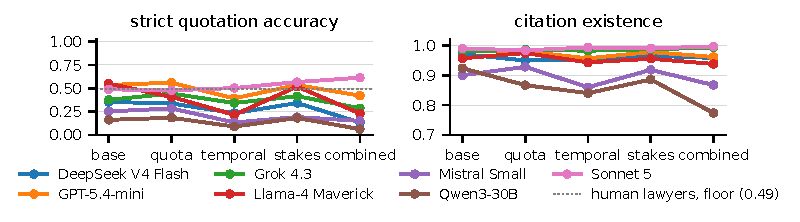
\includegraphics[width=\textwidth]{fig1_pressure.pdf}
\caption{Strict quotation accuracy (left) and citation existence (right) by condition, one line per model. The dotted line is the human-lawyer reference under the identical instrument. The right panel's axis starts at 0.7.}
\end{figure}

\begin{table}[t]
\caption{Baseline versus the combined condition, rows ordered by baseline strict quotation accuracy. Quotation columns give the strict rate with the lenient rate in parentheses; existence columns give the rate with the raw count of citations not found in brackets. An asterisk marks a contrast significant after Holm correction within model.}
\centering
\footnotesize
\begin{tabular}{llllll}
\toprule
Model & Quotes, base & Quotes, comb. & Exist, base & Exist, comb. & Temporal viol. \\
\midrule
Qwen3-30B & \strictQwenBase{} (\lenientQwenBase) & \strictQwenCombo{} (\lenientQwenCombo)$^*$ & \existQwenBase{} [\nfQwenBase] & \existQwenCombo{} [\nfQwenCombo]$^*$ & \violQwenTemporal\% \\
Mistral Small & \strictMistralBase{} (\lenientMistralBase) & \strictMistralCombo{} (\lenientMistralCombo) & \existMistralBase{} [\nfMistralBase] & \existMistralCombo{} [\nfMistralCombo] & \violMistralTemporal\% \\
DeepSeek V4 Flash & \strictDeepseekBase{} (\lenientDeepseekBase) & \strictDeepseekCombo{} (\lenientDeepseekCombo)$^*$ & \existDeepseekBase{} [\nfDeepseekBase] & \existDeepseekCombo{} [\nfDeepseekCombo] & \violDeepseekTemporal\% \\
Sonnet 5 & \strictSonnetBase{} (\lenientSonnetBase) & \strictSonnetCombo{} (\lenientSonnetCombo) & \existSonnetBase{} [\nfSonnetBase] & \existSonnetCombo{} [\nfSonnetCombo] & \violSonnetTemporal\% \\
Llama-4 Maverick & \strictLlamaBase{} (\lenientLlamaBase) & \strictLlamaCombo{} (\lenientLlamaCombo)$^*$ & \existLlamaBase{} [\nfLlamaBase] & \existLlamaCombo{} [\nfLlamaCombo] & \violLlamaTemporal\% \\
GPT-5.4-mini & \strictGptBase{} (\lenientGptBase) & \strictGptCombo{} (\lenientGptCombo) & \existGptBase{} [\nfGptBase] & \existGptCombo{} [\nfGptCombo] & \violGptTemporal\% \\
\bottomrule
\end{tabular}
\end{table}

\textbf{Citation existence.} Only the 30B model's existence moves under pressure: from \existQwenBase{} at baseline to \existQwenCombo{} under the combined condition, with the quota, temporal, and combined contrasts all significant after correction (combined OR \orCiteQwenCombo, corrected $p\,\holmCiteQwenCombo$). Mistral Small's existence sits between 0.86 and 0.93 across conditions and moves in the same direction without reaching significance; the four other models stay between 0.94 and 1.00 in every condition.

\textbf{Quotation accuracy.} The temporal restriction is the condition that damages quoting. After correction, strict quotation accuracy falls significantly under temporal and combined pressure for Qwen3-30B (\strictQwenBase{} to \strictQwenCombo) and Llama-4 (\strictLlamaBase{} to \strictLlamaCombo), and under the combined condition for DeepSeek (\strictDeepseekBase{} to \strictDeepseekCombo); GPT-5.4-mini and Mistral Small fall in the same direction without surviving correction, and Sonnet~5 does not fall at all. The Llama-4 row is the most consequential for practice: at baseline it quotes at the human reference level, \strictLlamaBase{} against \humanStrict, and under the temporal restriction its accuracy drops to \strictLlamaTemporal{} (OR \orQuoteLlamaTemporal, corrected $p\,\holmQuoteLlamaTemporal$). The lenient rates in Table~1 preserve the ordering, so the result does not depend on how bracketed alterations are scored.

\textbf{An exploratory contrast at the top.} Sonnet~5's strict quotation accuracy is numerically highest under the combined condition (\strictSonnetCombo{} against \strictSonnetBase{} at baseline; uncorrected $p=\pQuoteSonnetCombo$, corrected $p=\holmQuoteSonnetCombo$), and its citations not found went from \nfSonnetBase{} of \exSonnetBase{} at baseline to \nfSonnetCombo{} of \exSonnetCombo{}. Neither survives correction, the stakes condition alone moves neither outcome, and the temporal restriction changes the population of cited cases (median decision year 1943 under the combined condition against 1986 at baseline), so a shift toward well-memorized older opinions is an untested alternative to any reading in terms of care. We report the contrast because it appeared in the pre-registered analysis and draw no conclusion from it.

\textbf{Compliance with the temporal rule.} The share of checked citations that violate the pre-1970 restriction is \violQwenTemporal{} percent for Qwen3-30B, \violMistralTemporal{} percent for Mistral Small, between \violDeepseekTemporal{} and \violGptTemporal{} percent for the middle models, and \violSonnetTemporal{} percent for Sonnet~5 (one violation in 802 checked citations). Compliance improves with capability except for Mistral Small, which violates the rule most while its existence and quotation figures sit mid-table; compliance and fidelity are related but distinct. Zhao et al. found near-zero violations with fabrication filling the window; here the smaller models both fabricate and violate.

\textbf{Refusals and one model that stalls.} Across the \nPressured{} pressured drafts there were three refusals (two from DeepSeek, one from GPT-5.4-mini). GLM-4.7-flash produced no output on 30 of its 240 drafts, 23 of them in the combined condition, reasoning until a 30,000-token budget was exhausted in two escalating attempts. Because its missing drafts concentrate in the condition under comparison it is excluded from Table~1 and reported here as a failure mode the taxonomy should include: under stacked constraints some models neither fabricate nor refuse but stall.

\textbf{Robustness to phrasing.} The paraphrase arm was run on the four models available when it was designed. Under alternative phrasings of every condition on twelve matters, combined-condition existence was \paraParaExistQwenCombo{} for Qwen3-30B, \paraParaExistDeepseekCombo{} for DeepSeek, \paraParaExistGptCombo{} for GPT-5.4-mini, and \paraParaExistSonnetCombo{} for Sonnet~5, against \paraOrigExistQwenCombo, \paraOrigExistDeepseekCombo, \paraOrigExistGptCombo, and \paraOrigExistSonnetCombo{} on the same matters under the original phrasing. No existence result changes sign; quotation rates on twelve matters are too few to test and are given in the released data.

\section{Experiment 2: The Checker Inside the Revision Loop}

Combined-condition drafts entered a revision loop. Each round, the checker returned one line per failure (a citation that does not resolve; a quotation that does not appear verbatim in the cited opinion), the model revised, and the loop ended on a clean draft or after three revisions. A control with \textit{false feedback} gave the same number of identically formatted lines pointed at items that were correct. The loop used the first 24 matters in the pre-registered order (twelve per side). Loop rates are means over drafts, so round-0 figures differ slightly from the pooled rates of Table~1.

\begin{table}[t]
\caption{Revision under true checker feedback: scored quotations and accurate quotations before and after revision, strict accuracy, and episodes (of 24) that ended on a clean draft.}
\centering
\footnotesize
\setlength{\tabcolsep}{4pt}
\begin{tabular}{lcccccc}
\toprule
Model & \multicolumn{2}{c}{Quotes scored} & \multicolumn{2}{c}{Accurate} & Strict & Clean \\
 & r0 & final & r0 & final & r0 to final & \\
\midrule
Qwen3-30B & \lqScoredQwenTrueStart & \lqScoredQwenTrueFinal & \lqAccQwenTrueStart & \lqAccQwenTrueFinal & \loopQwenTrueStart{} to \loopQwenTrueFinal & \convQwenTrue \\
Mistral Small & \lqScoredMistralTrueStart & \lqScoredMistralTrueFinal & \lqAccMistralTrueStart & \lqAccMistralTrueFinal & \loopMistralTrueStart{} to \loopMistralTrueFinal & \convMistralTrue \\
DeepSeek V4 Flash & \lqScoredDeepseekTrueStart & \lqScoredDeepseekTrueFinal & \lqAccDeepseekTrueStart & \lqAccDeepseekTrueFinal & \loopDeepseekTrueStart{} to \loopDeepseekTrueFinal & \convDeepseekTrue \\
Sonnet 5 & \lqScoredSonnetTrueStart & \lqScoredSonnetTrueFinal & \lqAccSonnetTrueStart & \lqAccSonnetTrueFinal & \loopSonnetTrueStart{} to \loopSonnetTrueFinal & \convSonnetTrue \\
Llama-4 Maverick & \lqScoredLlamaTrueStart & \lqScoredLlamaTrueFinal & \lqAccLlamaTrueStart & \lqAccLlamaTrueFinal & \loopLlamaTrueStart{} to \loopLlamaTrueFinal & \convLlamaTrue \\
GPT-5.4-mini & \lqScoredGptTrueStart & \lqScoredGptTrueFinal & \lqAccGptTrueStart & \lqAccGptTrueFinal & \loopGptTrueStart{} to \loopGptTrueFinal & \convGptTrue \\
\bottomrule
\end{tabular}
\end{table}

\begin{figure}[t]
\centering
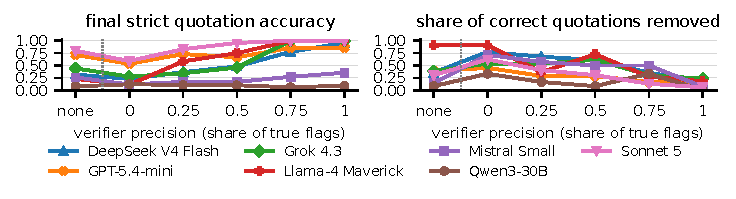
\includegraphics[width=0.75\textwidth]{fig2_repair.pdf}
\caption{Strict quotation accuracy from round 0 to the final draft under true feedback (solid) and false feedback (dashed), one color per model. A rate can rise because accurate quotations were added or because inaccurate ones were removed; Table~2 separates the two.}
\end{figure}

\textbf{Satisfying the checker by deletion.} Under true feedback the strict rate rises with capability, from \loopQwenTrueFinal{} for Qwen3-30B to \loopSonnetTrueFinal{} for Sonnet~5, and read alone this looks like repair. The counts in Table~2 say otherwise. Sonnet~5 went from \lqScoredSonnetTrueStart{} scored quotations to \lqScoredSonnetTrueFinal{} while its accurate quotations went from \lqAccSonnetTrueStart{} to \lqAccSonnetTrueFinal; the rate rose because the denominator collapsed. Told that a quotation was not verbatim, the model removed the quotation, or its quotation marks, far more often than it corrected the words. GPT-5.4-mini and DeepSeek show the same pattern. Qwen3-30B changed nothing: \lqScoredQwenTrueStart{} scored quotations became \lqScoredQwenTrueFinal{}, and \lqAccQwenTrueStart{} accurate ones stayed at \lqAccQwenTrueFinal. Citation existence, by contrast, was repaired rather than avoided: citation counts were flat (\lCitesSonnetTrueStart{} to \lCitesSonnetTrueFinal{} for Sonnet~5, \lCitesQwenTrueStart{} to \lCitesQwenTrueFinal{} for Qwen3-30B) while existence rose, so unresolvable citations were replaced with real ones. This answers the question the introduction asked. A checker in the revision loop does not, at any capability we tested, turn misquotations into quotations; it turns them into paraphrase or silence, which the checker cannot see and which a reader cannot distinguish from a brief that was never wrong.

\textbf{False feedback.} Under false feedback, four of six models ended with lower strict accuracy than they started, and the two weakest were unchanged within noise (Qwen3-30B \loopQwenScrStart{} to \loopQwenScrFinal, Llama-4 \loopLlamaScrStart{} to \loopLlamaScrFinal). The strongest models were harmed most: Sonnet~5 fell from \loopSonnetScrStart{} to \loopSonnetScrFinal{} and its accurate quotations from \lqAccSonnetScrStart{} to \lqAccSonnetScrFinal; GPT-5.4-mini fell from \loopGptScrStart{} to \loopGptScrFinal. Told that a correct quotation was wrong, a capable model rewrote it into something wrong. Our checker's own false-alarm rate on Sonnet~5's drafts was \falseAlarmSonnet{} verdicts in 240 drafts, low enough not to trigger this effect; a probabilistic detector with a false-positive rate in the tens of percent would trigger it, and intermediate rates were not tested.

\section{Residual Errors in the Strongest Models}

Three error classes remain when fabrication is rare, each measured deterministically on all six models.

\textbf{Paraphrase inside quotation marks.} Decomposing every inaccurate quotation against the cited opinion's own text, \decompParaPctSonnet{} percent of Sonnet~5's inaccurate quotations (\decompParaSonnet{} of them) are recognizable paraphrases of the correct case presented as verbatim quotation, \decompFabSonnet{} match nothing substantial in the cited opinion, and \decompOutSonnet{} cite authority outside the corpus's scope; GPT-5.4-mini's split is \decompParaPctGpt{} percent paraphrase. The characteristic error at the top of the range is not an invented case but quotation marks around a summary.

\textbf{Real language, wrong case.} Searching every inaccurate quotation against a segmented corpus of 8,392 Supreme Court opinions locates \misattrTotal{} quotations across the six models (\misattrSonnet{} for Sonnet~5, \misattrQwen{} for Qwen3-30B) whose distinctive language appears verbatim in a different opinion than the one cited. Because the attribution rule could itself misassign a quotation, the same search serves as an audit of the checker: it classified \falseAlarmSonnet{} of Sonnet~5's inaccurate verdicts and \falseAlarmQwen{} of Qwen3-30B's as the checker's own error, where the language was in the attributed case after all. A further screen for models reproducing the argued case's own later-decided opinion from memory found 41 candidates, of which 32 were record or statute text present in the prompt and the rest doctrinal formulas that the argued opinions were themselves quoting; the finding was withdrawn and is recorded in the ledger.

\textbf{Right case, wrong page.} Where a pinpoint and a quotation co-occur on a U.S. Reports authority, the quotation lies on the cited page \pinAtSonnet{} percent of the time for Sonnet~5, \pinAtGpt{} percent for GPT-5.4-mini, \pinAtDeepseek{} percent for DeepSeek, \pinAtLlama{} percent for Llama-4, \pinAtMistral{} percent for Mistral Small, and \pinAtQwen{} percent for Qwen3-30B, with pins outside the cited case rare at every tier. This measures on public data the error class that detection agents handle worst.

\textbf{Relevance judging: three failed calibrations.} Whether a real, correctly quoted case supports the proposition it is cited for cannot be looked up. We tried to calibrate language-model panels against the expert-labeled content-misrepresentation items of Liu et al. with a pre-declared bar of 0.75 accuracy on decisive verdicts: a three-model budget panel scored 0.500 with a binary verdict, 0.700 with a three-way verdict and abstention (misrepresentation recall 2 of 11), and a frontier panel of GPT-5.4, Sonnet~5, and Gemini 2.5 Pro with 15,000-character grounded excerpts scored 0.594 (recall 4 of 17). No measurement verdict from a failed panel was interpreted; relevance is a stated limitation of this work.

\section{Discussion}

The pressure results reorganize the question. Whether a model fabricates legal citations under realistic prompting has no single answer; it depends on the model, and the dependence runs against deployment economics, since cost pushes production toward the tier where a quota and an authority restriction triple the odds of a nonexistent citation. Quotation accuracy is more fragile than existence at every tier but the top, and the temporal restriction is the condition that breaks it, which matters because restricting authority by date or jurisdiction is a routine instruction.

The revision results carry the practical conclusions. A deterministic checker fed back into revision does not produce corrected quotations; it produces fewer quotations. For a supervising attorney that is not nothing, since a brief with fewer verbatim claims exposes fewer false ones, but it is not the repair a verification loop appears to promise, and a reader of the revised brief cannot tell which claims were demoted to paraphrase. The checker is more useful as a gate on output, holding a draft until its citations resolve and its quotations match, than as feedback the model may satisfy by avoidance. Any system that feeds a probabilistic detector's flags to a capable model should measure the detector's false-positive rate first, because the models that follow feedback best are the ones a false flag damages most.

For courts and regulators, the instrument matters as much as the findings. Existence, verbatim quotation, and pinpoint page can be checked deterministically from public data, and the released verifier does so; standing orders that require disclosure of AI assistance could additionally require the checker's output on the filing. What cannot yet be checked is whether a real citation supports the proposition, and no language-model jury we assembled met a modest validity bar on that question. With retrieval-grounded tools we expect existence failures to shrink further and the residual classes, paraphrase in quotation marks and wrong pages, to remain, since they arise in composition rather than recall.

\section{Limitations}

Single domain and single task: Supreme Court merits argument, one packet format, one fixed template per condition with a phrasing check on twelve matters rather than a full paraphrase factorial. The task is closed-book, which matches the sanctioned filings but not commercial legal tools. The stakes clause names a sanctions rule that does not govern the forum. The strict verbatim standard penalizes bracketed alterations and ellipses for humans and models alike, and the human reference differs from the model drafts in citation mix. The provenance corpus covers 8,392 Supreme Court opinions and cannot adjudicate quotations from other courts. The false-feedback control is all false; intermediate false-positive rates and a no-feedback revision control were run after the pre-registered analysis and are reported in the released data rather than here. Inference is per model at 48 matters, the independent units the clustering respects, so effects of a few points are not detectable, and the six-model set is one model per vendor rather than a sampled population, so capability, family, and training recipe are confounded.

\section{Conclusion}

Under the prompting pressures users actually apply, citation integrity degrades from the smallest model upward: nonexistent citations at 30B, misquotation through the middle of the range, and misattribution and wrong pages at the top. A deterministic checker built from public data sees all of this. Fed back into revision it produces briefs with fewer quotations rather than corrected ones, and false feedback corrupts the models that listen. The instruments, the seeded-fault validation harness, the forking-paths ledger, and per-citation records for every table are released so that the checks can be run on any brief.

\section{Ethics and Release}

All source material is public court data. Drafts were generated for measurement and none was filed. Code, instruments, drafts, and records are at \texttt{github.com/\allowbreak hardy30894/\allowbreak citation-under-pressure}. Language-model assistance was used in writing code and prose under the author's direction; every reported number is produced by the released deterministic instruments.

\bibliographystyle{vancouver}
\bibliography{references,ailaw}

\end{document}
